\chapter{A Static Scheduling Language for Parallel Tree Traversals}
\label{chap:3}

We now introduce a static scheduling language for parallel computations over a tree such as those seen in layout. A compiler takes an attribute grammar (the functional specification) and its schedule and outputs an implement, i.e., a layout engine. For now, we ignore the source of the schedule. Beyond presenting the language and compilation strategy, we show how to verify functional and behavioral (parallel) correctness, introduce the first parallel schedule for a large subset of CSS, and show how, on GPU tree computations, memory may be dynamically allocated quite efficiently.

The goal of our language for traversals over trees is to benefit from high-performance computing techniques  commonly used for stencils over grids. Common for physical modeling, a stencil computation is one where a kernel only reads and writes to a limited set of nodes, there are many kernels, and the data dependencies between kernels lead to traversal patterns such as a wavefront. Many variants of stencils exist. The enthusiasm for them stems from programmers or stencil compilers being able to exploit knowledge of their structure to effectively optimize for use of cache lines, memory, parallel processors, and other resources. Similar techniques are known for trees, and the next chapter introduces additional ones.

Our first challenge in this chapter is to restrict the scheduling language enough to facilitate optimization while still providing the flexibility for expressing  document layout and data visualization workloads. Finding parallelism in CSS is already novel,  so being further able to optimize it with techniques associated with small formulas for physical models is surprising. We found that, while layout computations have too many data dependencies to be solved with one simple tree traversal, sequences of 3--5 traversals often suffice for data visualizations and 9 for CSS. Our scheduling language therefore consists of traversal patterns, such as parallel top down (\emph{preorder}) traversal of the tree, and ways of combining them, such as in a sequence. One especially representative case study of matching restrictions with flexibility was in our study of  visualizations: dynamic memory allocation on a GPU is generally a bottleneck, but we used a sequence of tree traversals for parallel allocation of render buffers for each node.

Another artifact of layout specifications being magnitudes bigger than stencil formulas is that the correctness concerns change. For stencil computations, the verification challenge lies more in correctly optimizing the implementation of a traversal schedule. Layout computations encounter a challenge before that point: the size of the functional specification and the ensuing tangle of data dependencies require ensuring  that the parallel schedule itself is safe to implement. We use a variant of existing static dependency analyses of attribute grammars to verify that the schedule is race-free. 


The dependencies that complicate reasoning about correctness of parallel code actually also complicate sequential code. Our use of static analysis for the attribute grammars leads to an important result for layout languages: we show how to statically verify three important properties about them.  
\begin{itemize}
\item \textbf{Totality} The layout language defines a solution for every syntactically well-formed input tree; it is unambiguous. 
\item \textbf{Determinism} As discussed  in the previous paragraph, parallelization is safe.
\item \textbf{Linearity (Single Assignment)} Every attribute is assigned to exactly once. Layout languages often perform \emph{reflow} to iteratively solve constraints or incremental computation, so this property bounds the need for it. 
\end{itemize}
The first property demonstrates the ability to reason about \emph{functional correctness} and the last two about \emph{behavioral correctness}. Put together, we verify that a language is unambiguous, supports parallelization, and with bounded asymptotic complexity.  

\section{Language of Static Schedules}
%Our approach builds upon the ideas of multipass attribute grammars and statically ordered attribute grammars~\cite{oag}. Before showing our technique, we review how to use these ideas on how to more efficiently evaluate attribute grammars than the na\"{i}ve dynamic approach of Chapter~\ref{chap:2}. Furthermore, we review how they enable proving properties about the attribute grammars such as unambiguity, and (inefficient) parallelization strategies. 

This section focuses on defining our full language of traversal schedules. It is the input for our code generators. Programmers either do not specify the schedule in practice due to our automation support, or use the \emph{sketching} extension (Section~\ref{sec:holes}) for more succinct partial specification.

Statically scheduled evaluation departs from the dynamic evaluation strategy of Chapter~\ref{chap:2}. Static scheduling solves the performance problem of dynamic evaluation repeatedly manipulating the data dependencies of every attribute at runtime. For example, what would be a direct sequence of arithmetic statements in a static language becomes an interleaving of graph manipulations and arithmetic with the dynamic evaluator. The runtime scheduling overhead for evaluating all the statement is (at least) linear in the size of the data dependency graph. 

Instead, a schedule statically specifies most of the scheduling decisions.  It specifies a sequence of tree traversals and the order of statements to use within each traversal. During a traversal at runtime, the order of nodes to traverse is based on the traversal pattern, such as top-down, rather than by inspecting data dependencies. Likewise, the statements to execute for a node are looked up based on the node's type rather than by data dependencies.  Our approach is a more compositional variant of others. Our flexibility requirements led to focusing on the ability to compose different types of traversals, such as by sequencing and nesting.


\newsavebox{\seqtraversals}
\begin{lrbox}{\seqtraversals}% Store first listing
\begin{minipage}{1\columnwidth}
\begin{lstlisting}[mathescape,language=C++,morekeywords={spawn,join}]
void preorder(void (*visit)(Prod &), Prod &p) {
  visit(p);
  for (Prod rhs in p) 
    preorder(visit, rhs);
}
void postorder(void (*visit)(Prod &), Prod &p) {
  for (Prod rhs in p) 
    postorder(visit, rhs);
  visit(p);
}
void recursive(void (*visit)(Prod &, int), Prod &p) {
    int step = 0;
    visit(p, step++);
    for (Prod rhs in p) {
      recursive(visit, rhs);
      visit(p, step++); //repeat visit to p
    }
}
\end{lstlisting}
\end{minipage}
\end{lrbox}

\newsavebox{\seqtraversalsequence}
\begin{lrbox}{\seqtraversalsequence}% Store first listing
\begin{minipage}{1\columnwidth}
\begin{lstlisting}[mathescape,language=C++,morekeywords={spawn,join}]
postorder(visit1, start); 
preorder(visit2, start);
\end{lstlisting}
\end{minipage}
\end{lrbox}


\newsavebox{\hboxvisitors}
\begin{lrbox}{\hboxvisitors}% Store first listing
\begin{minipage}{1\columnwidth}
\begin{lstlisting}[mathescape,language=C++]
void visit1 (Prod &p) {
  switch (p.type) {
    case S $\rightarrow$ HBOX:  break;
    case HBOX $\rightarrow$ $\epsilon$:
      HBOX.w = input(); HBOX.h = input(); break;
    case HBOX $\rightarrow$ HBOX$_1$ HBOX$_2$:
      HBOX$_0$.w = HBOX$_1$.w + HBOX$_2$.w;
      HBOX$_0$.h = MAX(HBOX$_1$.h, HBOX$_2$.h);
      break;
  }
}
void visit2 (Prod &p) {
  switch (p.type) {
    case S $\rightarrow$ HBOX:
      HBOX.x = input(); HBOX.y = input(); break;
    case HBOX $\rightarrow$ $\epsilon$: break;
    case HBOX $\rightarrow$ HBOX$_1$ HBOX$_2$:
      HBOX$_1$.x = HBOX$_0$.x;
      HBOX$_2$.x = HBOX$_0$.x + HBOX$_1$.w;
      HBOX$_1$.y = HBOX$_0$.y;
      HBOX$_2$.y = HBOX$_0$.y;
      break;
  }
}
\end{lstlisting}
\end{minipage}
\end{lrbox}




\begin{figure}
\subfloat[\textbf{Sequential sequence of traversals}]{\label{fig:hboxseq:sequence} \usebox{\seqtraversalsequence} } \\
\subfloat[\textbf{Three sequential traversal patterns}]{\label{fig:hboxseq:traversals} \usebox{\seqtraversals} } \\
\subfloat[\textbf{Scheduled and compiled visits for ~\hlang{}.}]{\label{fig:hboxseq:compiled} \usebox{\hboxvisitors} } \\
\caption{\textbf{Sequentially scheduled and compiled layout engine for \hlang{}.}}
\label{fig:hboxseq}
\end{figure}





\subsection{Sequential Schedules}  
\label{subseq:seqscheds}
We start by examining how to specify a safe static schedule for \hlang that respects any possible dynamic dependencies (Figure~\ref{fig:deps:full}).
%Research into statically scheduled sequential attribute grammars revealed a variety of scheduling options. For example, some computations can be solved in one traversal over a tree and therefore merged into a parser, while others require multiple traversals. We focus on several important options and the automated reasoning supported for them.

Figure~\ref{fig:hboxseq} shows a sequential implementation of \hlang decomposed into several pieces. The layout engine solves an input tree over a sequence of two traversals (Figure~\ref{fig:hboxseq:sequence}). The first traverses the tree in postorder, meaning from the leaves up to the root (''bottom-up'') and the second performs are preorder traversal, meaning from the root down to the leaves (''top-down''). Figure~\ref{fig:hboxseq:traversals} provides a sample implementation of generic traversal code. During a during traversal, each node is \emph{visited} exactly once in order to compute the attributes whose dependencies have been satisfied. Figure~\ref{fig:hboxseq:compiled} shows that the first pass computes widths and heights and the second pass computes the x and y positions.

The example follows a static schedule rather than manipulating a dynamic data dependency graph. The sequence of traversal invocations and the code used for the different cases for each traversal's visitor determine the schedule. Each traversal now only performs dynamic scheduling in the sense of maintaining a stack for recurring down the tree, which is a cost proportional to the number of nodes rather than the size of the dynamic dependency graph between attributes. In practice (Chapter~\ref{chap:6}), our compiler and runtime optimizations even eliminate the example's implicit use of a call stack.


The decompose the schedule into several types of policy fragments. First, the schedules involves a \emph{sequence} of  \emph{two different types} of traversals:
\begin{lstlisting}
      postorder(visit1, start); preorder(visit2, start)
\end{lstlisting}
Just one bottom-up traversal cannot compute all the attributes, such as all the x and y attributes that flow downwards (Figure~\ref{fig:deps:full}), so the schedule may require multiple types of traversals and in a careful order.  Furthermore, within a traversal, the schedule specifies different orders of statements for different types of nodes. Consider the following fragment:
\begin{lstlisting}
      HBOX$_1$.x = HBOX$_0$.x;
      HBOX$_2$.x = HBOX$_0$.x + HBOX$_1$.w;
\end{lstlisting}
The schedule specifies that \code{HBOX}$_2$\code{.x} can (and should) be immediately evaluated after \code{HBOX}$_1$\code{.x} without fear of unsatisfied data dependencies for any of its right-hand side terms. In summary, we see three parts to a schedule: the staging of traversals, the node visit order for every individual traversal, and the statement order for different types of nodes within a specific traversal.

We abstracted the three aspects of a schedule into a scheduling language (Figure~\ref{fig:hboxparallel}). For example, the schedule for the above computation would be appear as:
\begin{lstlisting}[mathescape,morekeywords={preorder,postorder}]
postorder
  HBOX$_0$ $\rightarrow$ HBOX$_1$ HBOX$_2$ { HBOX$_0$.w HBOX$_0$.h }
  HBOX $\rightarrow$ $\epsilon$ { HBOX.w HBOX.h }
;
preorder
  S $\rightarrow$ HBOX { HBOX.x HBOX.y }
  HBOX$_0$ $\rightarrow$ HBOX$_1$ HBOX$_2$ 
    { HBOX$_1$.x HBOX$_2$.x HBOX$_1$.y HBOX$_2$.y }
\end{lstlisting}
It specifies a sequence ('';'') of two traversals of node visit order \code{postorder} and \code{preorder}. For each type of node visited within a traversal, the schedule specifies the sequential sequence of attributes to evaluate. We note that, due to the desugaring of our class system in Section~\ref{sec:desugaring}, the dispatches in the above examples are based on grammar productions in the desugared representation. In terms of the fronted language, the dispatches are based on node class.


Generally, a single attribute grammar may be schedule in many ways. For example, the width and height computations share no dependencies, so the first postorder traversal might be partitioned into two postorder traversals:
\begin{lstlisting}[mathescape,morekeywords={preorder,postorder}]
postorder
  HBOX$_0$ $\rightarrow$ HBOX$_1$ HBOX$_2$ { HBOX$_0$.w }
  HBOX $\rightarrow$ $\epsilon$ { HBOX.w }
;
postorder
  HBOX$_0$ $\rightarrow$ HBOX$_1$ HBOX$_2$ { HBOX$_0$.h }
  HBOX $\rightarrow$ $\epsilon$ { HBOX.h }
;
preorder
  S $\rightarrow$ HBOX { HBOX.x HBOX.y }
  HBOX$_0$ $\rightarrow$ HBOX$_1$ HBOX$_2$ 
    { HBOX$_1$.x HBOX$_2$.x HBOX$_1$.y HBOX$_2$.y }
\end{lstlisting}
Rescheduling in this way may improve performance on small devices with little memory because the schedule cuts the working set size in half for each traversal. Note, however, that the schedule only optimizes execution; it does not change the result of evaluation.


\begin{figure}
\centering
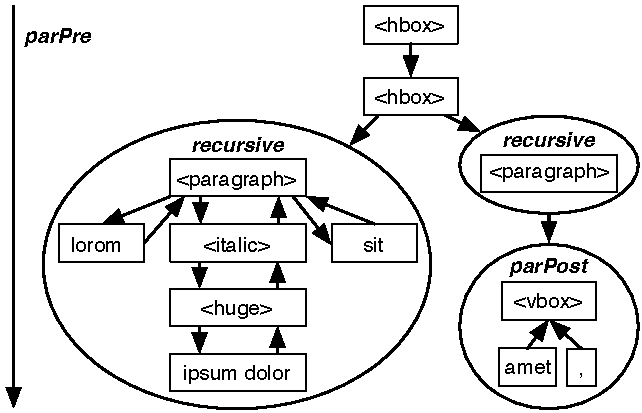
\includegraphics[trim=0 0 0 0,clip,width=0.7\columnwidth]{chapter3/nested}
\caption{\textbf{Nested traversal for line breaking}. The two paragraphs are traversed in parallel as part of a preorder traversal. A sequential recursive traversal places the words within a paragraph. Circles denote nested regions and arrows show data dependencies between nodes and/or regions.}
\label{fig:nested}
\end{figure}

Sequential execution supports a traversal type that can compute more than \code{postorder} or \code{preorder}, which we call a \code{recursive} traversal (Figure~\ref{fig:hboxseq:traversals}). We use a recursive traversal, for example, for line breaking in our document layout case study. Consider inserting line breaks into the following stylized paragraph of XML strings (Figure~\ref{fig:nested}):
%
$$\texttt{lorom <italic><huge>ipsum dolor</huge></italic> sit}$$
%
Due to \texttt{<huge>}, the paragraph may need a line break between ``ipsum'' and ``dolor.''  Identifying the line break position involves visiting the subtree  \texttt{<italic>...</italic>}; the resulting line break position is a data dependency influencing line breaks in the remainder of the text. The sequence of arrows in the big circle of Figure~\ref{fig:nested} show a trace of performing a recursive traversal over the paragraph. The traversal visits a node $n$, then visits $n$'s first child, revisits $n$, and repeats this process for the remaining children before returning to the parent. 

The relationship between \code{recursive} traversals and \code{postorder} and \code{preorder} merits examination. First, a sequence of a preorder traversal followed by a postorder traversal may be merged into one recursive traversals. Traversing a tree induces overhead costs, so such fusion may be beneficial. The reverse  relationship is not true, however. As happens with the case of line breaking, long-running sequential dependencies may prevent splitting a recursive traversal into a preorder and postorder traversal. These dependencies arise because the the same node is visited multiple times in a traversal: once before a child subtree is traversed and again after. The result of computing over one subtree may therefore be used to compute another, which supports long-running sequential dependencies. 


\newsavebox{\decomplang}
\begin{lrbox}{\decomplang}% Store first listing
\begin{minipage}{1\columnwidth}
\renewcommand{\litleft}{\bfseries}
\renewcommand{\ulitleft}{\bfseries}
\renewcommand{\superscript}[1]{\ensuremath{^{\textrm{#1}}}}
\renewcommand{\subscript}[1]{\ensuremath{_{\textrm{\uppercase{#1}}}}}
\renewcommand{\syntleft}{\normalfont\itshape\texttt{<}}
\renewcommand{\syntright}{\texttt{>}}
\begin{grammar}
<Sched> \deriv{} <Sched> ; <Sched>  ~ | ~ <Sched> $\vert\vert$ <Sched>  ~|~ <Trav>

<Trav> \deriv{} <TravAtomic> <Visit>*\{(<TravAtomic> $\mapsto$ <Visit>*)*\}?

<TravAtomic>  \deriv{} "preorder" ~ | ~ "postorder" ~ | ~ "parPre"  ~ | ~  "parPost"  ~ | ~  "recursive" ~ 

<Visit> \deriv{} <Prod>  \{ <Step>* \}

<Step> \deriv{} \emph{attrib} ~ | ~ "recur" \emph{v}
\end{grammar}
%<Sched, Trav, Visit, Step> \deriv{} \ldots ~ | ~ $\hole$        
\end{minipage}
\end{lrbox}


\newsavebox{\hboxdecomp}
\begin{lrbox}{\hboxdecomp}% Store first listing
\begin{minipage}{1\columnwidth}
\begin{lstlisting}[mathescape,morekeywords={parPre,parPost}]
parPost
  HBOX$_0$ $\rightarrow$ HBOX$_1$ HBOX$_2$ { HBOX$_0$.w HBOX$_0$.h }
  HBOX $\rightarrow$ $\epsilon$ { HBOX.w HBOX.h }
;
parPre
  S $\rightarrow$ HBOX { HBOX.x HBOX.y }
  HBOX$_0$ $\rightarrow$ HBOX$_1$ HBOX$_2$ 
    { HBOX$_1$.x HBOX$_2$.x HBOX$_1$.y HBOX$_2$.y }
\end{lstlisting}
\end{minipage}
\end{lrbox}

\newsavebox{\traversals}
\begin{lrbox}{\traversals}% Store first listing
\begin{minipage}{1\columnwidth}
\begin{lstlisting}[mathescape,language=C++,morekeywords={spawn,join}]
void parPre(void (*visit)(Prod &), Prod &p) {
  visit(p);
  for (Prod rhs in p) 
    spawn parPre(visit, rhs);
  join;
}
void parPost(void (*visit)(Prod &), Prod &p) {
  for (Prod rhs in p) 
    spawn parPost(visit, rhs);
  join;
  visit(p);
}
\end{lstlisting}
\end{minipage}
\end{lrbox}

\newsavebox{\hboxparvisitors}
\begin{lrbox}{\hboxparvisitors}% Store first listing
\begin{minipage}{1\columnwidth}
\begin{lstlisting}[mathescape,language=C++]
parPost(visit1, start); parPre(visit2, start);
\end{lstlisting}
\end{minipage}
\end{lrbox}


\begin{figure}
\subfloat[\textbf{One explicit parallel schedule for ~\hlang{}.}]{\label{fig:hboxparallel:schedule} \usebox{\hboxdecomp} } \\
\subfloat[\textbf{Na\"{\i}ve traversal implementations} with Cilk's~\cite{cilk} \sched{spawn} and \sched{join}.]{\label{fig:hboxparallel:traversals} \usebox{\traversals} } \\
\subfloat[\textbf{Scheduled and compiled layout engine for ~\hlang{}.}]{\label{fig:hboxparallel:compiled} \usebox{\hboxparvisitors} } \\
\subfloat[\textbf{Language of schedules} (without holes) ]{\label{fig:hboxparallel:decomplang} \usebox{\decomplang} }
\caption{\textbf{Scheduled and compiled layout engine for \hlang{}.}}
\label{fig:hboxparallel}
\end{figure}




\begin{figure}
\subfloat[First traversal: parallel postorder]{\label{fig:depsparallel:postorder}
\begin{minipage}{0.5\columnwidth}\centering
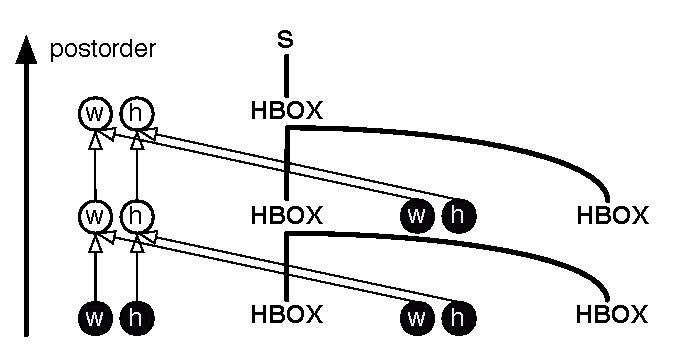
\includegraphics[trim=0 0 0 0,clip,width=1.0\columnwidth]{chapter3/depspostorder}
\end{minipage}}
\subfloat[Second traversal: parallel preorder.]{\label{fig:depsparallel:preorder}
\begin{minipage}{0.5\columnwidth}\centering
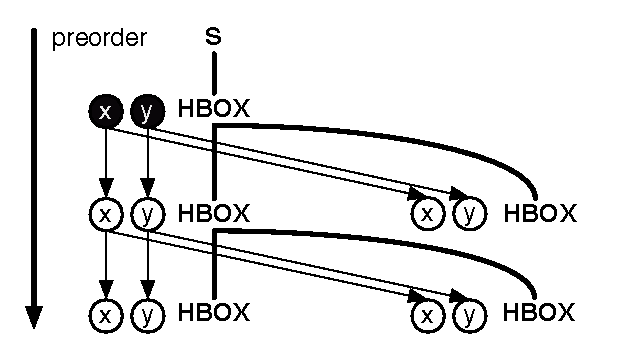
\includegraphics[trim=0 0 0 0,clip,width=1.0\columnwidth]{chapter3/depspreorder}
\end{minipage}}
\caption{\textbf{Parallel Traversal}. Shown for constraint tree  in Figure~ZZZ~(a). Circles denote attributes, with black circles denoting attributes with resolved dependencies such as \sched{input()}s. Thin lines show data dependencies and thick lines show production derivations. First diagram shows dependencies followed by first traversal, and second for the following traversal.}
\label{fig:depsparallel}
\end{figure}


\subsection{Parallel Schedules: Same Traversal}
A schedule exposes structured parallelism both within a traversal and across them. 

For an example of parallelism within a traversal, the first postorder traversal for \hlang features latent parallelism. The widths and heights for one subtree can be computed independently of the widths and heights of another distinct subtree. Figure~\ref{fig:depsparallel:postorder} shows an example where different (logical) threads may compute on the leaf nodes and implicit barriers force a join at every intermediate node. Likewise, the second traversal (Figure~\ref{fig:depsparallel:preorder}) may be changed to a parallel preorder traversal where ever intermediate node acts as a logical fork. Figure~\ref{fig:hboxparallel:traversals} depicts na\"{i}ve parallel implementations using Cilk's~\cite{??} \code{spawn} and \code{join} primitives. We formulate the schedule by changing the specification from \code{postorder} and \code{preorder} to \code{parPost} and \code{parPre} (Figure~\ref{fig:hboxparallel:schedule}).


Our \emph{nested} traversal feature supports exploiting parallelism within a traversal even if some nodes require sequential evaluation.  With it, the tree is partitioned into an outer region and disjoint inner regions.  The outer and inner regions are evaluated with different traversals, and both may exploit parallelism.  We can think of the inner regions as macro-nodes that are evaluated in full (with their particular traversal type) when the outer traversal encounters them.  

To motivate the need for nested traversals, we revisit line breaking.  Even though line breaking of a single paragraph is sequential, distinct paragraphs of text can be handled in parallel.  To avoid locally sequential computations from forcing the entire tree traversal to be sequential, we allow the outer region to be parallel, while each paragraph forms an inner region that is handled with the sequential recursive traversal. Figure~\ref{fig:nested} shows how parallel evaluation may be used to compute across different \sched{recursive} paragraphs. Likewise, it shows a hypothetical \code{VBox} subtree that uses parallel postorder evaluation for traversing its subtree as soon as the outer parallel preorder traversal reaches it.

%A nested traversal supports parallelism. First, the outer traversal may itself be parallel, such as the two paragraphs in Figure~\ref{fig:nested} being evaluated concurrently as part of an overall preorder traversal. Second, each macro-node may itself be evaluated with a parallel traversal internally whenever the outer traversal reaches it. For example, parallel evaluation may be used within the preorder and postorder macro-nodes in Figure~\ref{fig:nested}.

To partition a tree into regions, the schedule maps each grammar production (and thus each node of the tree) to a traversal type in the synthesized schedule.  A subtree composed from nodes of the same traversal types form an inner region.  For example, a nested traversal of paragraphs with sequential traversals of nested text subtrees is described as follows: 

\begin{lstlisting}[mathescape,morekeywords={parPre,parPost,nested,recursive,recur}]
parPre 
  P $\rightarrow$ W { W.relativeX }
  { recursive $\mapsto$   
      W$_0$ $\rightarrow$ W$_1$ W$_2$ {
        W$_1$.relativeX recur W$_1$ 
        W$_2$.relativeX recur W$_2$ } }
\end{lstlisting}


\subsection{Parallel Schedules: Across Travesals}
We may exploit parallelism across traversals as well. For example, just as we created a different but functionally equivalent sequential schedule for \hlang, we can do the same manipulation to yield a new parallel schedule:

\begin{minipage}{1\columnwidth}
\begin{lstlisting}[mathescape,morekeywords={parPre,parPost}]
(   parPost
     HBOX$_0$ $\rightarrow$ HBOX$_1$ HBOX$_2$ { HBOX$_0$.w }
     HBOX $\rightarrow$ $\epsilon$ { HBOX.w }  
   $||$  
    parPost
     HBOX$_0$ $\rightarrow$ HBOX$_1$ HBOX$_2$ { HBOX$_0$.h }
     HBOX $\rightarrow$ $\epsilon$ { HBOX.h })
; parPre $\ldots$ $\emph{/* same as before */}$
\end{lstlisting}
\end{minipage}
The ``$||$'' construct specifies that one traversal may be run concurrently with another. Neither traversal traversal depends on attributes written by the other, so the parallelizaton is safe. Even if we cannot exploit parallelism within a traversal, using ``$||$'' enables us to exploit parallel across them. 









\subsection{Compilation}
Compilation only requires an attribute grammar and the schedule. The traversal staging \code{postorder _ ; preorder _} directly translates to the executable fragment in Figure~\ref{fig:hboxseq:sequence}. Likewise, the mapping from traversal productions to statement sequences, such as \code{HBOX} $\rightarrow \epsilon$ \{ \code{HBOX.w HBOX.h} \}, directly translate to the visit functions of Figure~\ref{fig:hboxseq:compiled}. The translation matches an attribute in the schedule with the lefthand side attribute of an equation in the attribute grammar and outputs the full assignment statement in its place. 

Our code generation pipeline is further complicated but conceptually similar. The schedule is combined with the attribute grammar to form an intermediate representation, and different code generators target different backends such as JavaScript, OpenCL, and C++. Furthermore, some of the reductions of Section~\ref{sec:desguaring} require augmenting or rewriting the intermediate representation, such as reinserting loops that were unrolled during scheduling (Section~\ref{???}). Our end-to-end compiler design is slightly different due to the synthesis algorithm (Chapter~\ref{chap:4})  and schedule autotuning (Section~\ref{sec:schedtuning}), but code generation for a schedule follows a more conventional process.


\section{Automatically Staging Memory Allocation for SIMD Rendering}
\newsavebox{\stagedAllocFull}
\begin{lrbox}{\stagedAllocFull}% Store first listing
\begin{lstlisting}[mathescape]
float *drawCircle (float x, float y, float radius) {
  float *buffer = malloc( (2 * sizeof(float) ) * round(radius))
  for (int i = 0; i < round(radius); i++) {
    buffer[2 * i] = x + cos(i * PI/radius);
    buffer[2 * i + i] = y + sin(i * PI/radius);
  }
  return buffer;
}
\end{lstlisting}
\end{lrbox}

\newsavebox{\stagedAllocAlloc}
\begin{lrbox}{\stagedAllocAlloc}% Store first listing
\begin{lstlisting}[mathescape]
int allocCircle (float x, float y, float radius) {
  return round(radius);
}
\end{lstlisting}
\end{lrbox}


\newsavebox{\stagedAllocRender}
\begin{lrbox}{\stagedAllocRender}% Store first listing
\begin{lstlisting}[mathescape]
int fillCircle(float x, float y, float radius, float *buffer) {
  for (int i = 0; i < round(radius); i++) {
    buffer[2 * i] = x + cos(i * PI/radius);
    buffer[2 * i + i] = y + sin(i * PI/radius);
  }	
  return 0;
}
\end{lstlisting}
\end{lrbox}


\begin{figure}
\subfloat[\textbf{Na\i{v}e drawing primitive .}]{\label{fig:stagedalloc:original} \usebox{\stagedAllocFull} }  \\
\subfloat[\textbf{Allocation phase of drawing}.]{\label{fig:stagedalloc:alloc} \usebox{\stagedAllocAlloc} } \\
\subfloat[\textbf{Tessellation phase of drawing}.]{\label{fig:stagedalloc:use} \usebox{\stagedAllocRender} } 
\caption{\textbf{Partitioning of a library function that uses dynamic memory allocation into parallelizable stages.}}
\label{fig:stagedalloc}
\end{figure}


\newsavebox{\twocirclesOrig}
\begin{lrbox}{\twocirclesOrig}% Store first listing
\begin{lstlisting}[mathescape]
CBOX $\rightarrow$ BOX$_1$ BOX$_2$
{
  ...
  CBOX.render = 
    drawCircle(CBOX.x, CBOX.y, CBOX.radius)
      + drawCircle(CBOX.x + 10, CBOX.y + 10, CBOX.radius * 0.5);
}
\end{lstlisting}
\end{lrbox}

\newsavebox{\twocirclesExpanded}
\begin{lrbox}{\twocirclesExpanded}% Store first listing
\begin{lstlisting}[mathescape]
CBOX $\rightarrow$ BOX$_1$ BOX$_2$
{
  ...
  CBOX.sizeSelf = 
    allocCircle(CBOX.x, CBOX.y, CBOX.radius)
      + allocCircle(CBOX.x + 10, CBOX.y + 10, CBOX.radius * 0.5);
  CBOX.size = CBOX.sizeSelf +BOX$_1$.size + BOX$_2$.size;
  BOX$_1$.buffer = CBOX.buffer + CBOX.sizeSelf;
  BOX$_2$.buffer = BOX$_1$.buffer + BOX$_1$.size;
  CBOX.render = 
    fillCircle(CBOX.x, CBOX.y, CBOX.radius, CBOX.buffer)
      + fillCircle(CBOX.x + 10, CBOX.y + 10, CBOX.radius * 0.5,
            CBOX.buffer + allocCircle(CBOX.x, CBOX.y, CBOX.radius));
}
\end{lstlisting}
\end{lrbox}

\newsavebox{\twocirclesMacro}
\begin{lrbox}{\twocirclesMacro}% Store first listing
\begin{lstlisting}[mathescape]
CBOX $\rightarrow$ BOX$_1$ BOX$_2$
{
  ...
  CBOX.render = 
      @Circle(CBOX.x, CBOX.y, CBOX.radius)
      + @Circle(CBOX.x + 10, CBOX.y + 10, CBOX.radius * 0.5);
}
\end{lstlisting}
\end{lrbox}




\begin{figure}
\subfloat[\textbf{Call into inefficient library.}]{\label{fig:stagedallocClient:original} \usebox{\twocirclesOrig} }  \\
\subfloat[\textbf{Macro-expanded calls into staged library}.]{\label{fig:stagedallocClient:expanded} \usebox{\twocirclesExpanded} }  \\
\subfloat[\textbf{Sugared calls into staged library}.]{\label{fig:stagedallocClient:macro} \usebox{\twocirclesMacro} } 
\caption{\textbf{Use of dynamic memory allocation in a grammar for rendering two circles.}}
\label{fig:stagedallocClient}
\end{figure}

\begin{figure}
\centering
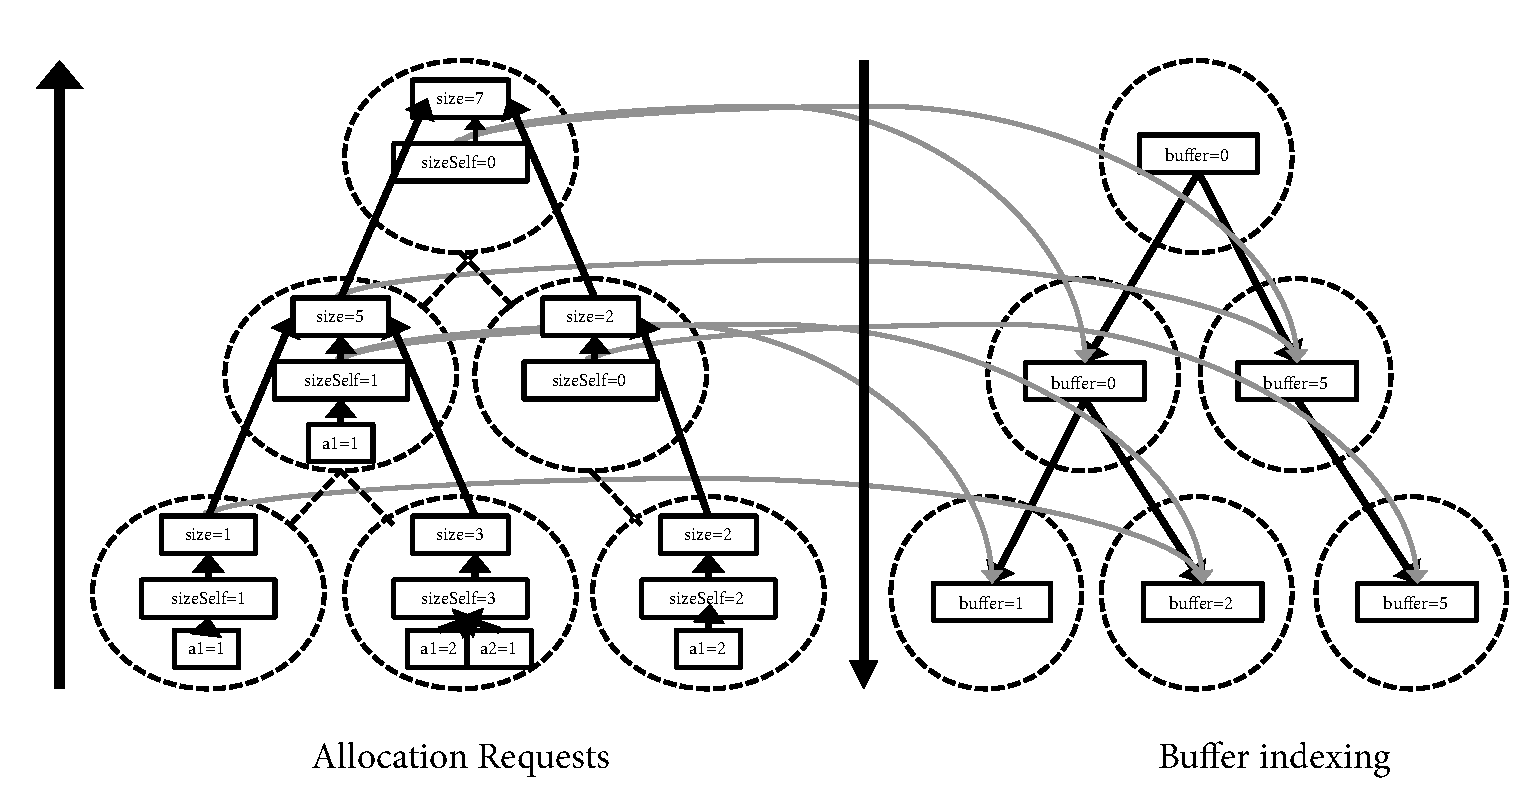
\includegraphics[trim=0 0 0 0,clip,width=1.0\columnwidth]{chapter6/macro}
\caption{\textbf{Staged parallel memory allocation as two tree traversals.} First pass is parallel bottom-up traversal computing the sum of allocation requests and the second pass is a parallel top-down traversal computing buffer indices. Lines with arrows indicate dynamic data dependencies.}
\label{fig:renderingtraversal}
\end{figure}


\subsection{Problem}
The static language of traversals is restricted, but we find that it can express important cases of typically more dynamic constructs. Prominent in our case studies, dynamic memory allocation provides significant flexibility for a language, but it is unclear how to perform it on a GPU without significant performance penalties. Our insight is that the memory allocation may be staged with parallel traversals by using a variant of prefix sum node labeling. One pass gathers  memory requests, a bulk allocation for the total amount is made, and then a scatter pass provides each node with a contiguous memory segment of it. We found manipulating memory addresses in this way to be error-prone, so we created two complementary automation techniques. First, we use our synthesizer to automatically schedule parallel memory allocation. Second, we syntactically hide the use of our optimization through a macro that automatically expands into staged dynamic memory allocation and consumption calls.

For example, we found parallel dynamic memory allocation to simplify the transition between layout and rendering. All nodes that render a circle will call some form of \code{drawCircle} in Figure~\ref{fig:stagedalloc:original}. Depending on the size of the circle, which is computed as part of the layout traversals, a different amount of memory will be allocated. Once the memory is allocated, vertices will be filled in with the correct position. The rendering engine will then connect the vertices with lines and paint them to the screen. The processing of converting the abstract shape into renderable vertices is known as tessellation. We want our system to tesselate the display objects for each node in parallel.




\subsection{Staged Parallel Memory Allocation}
We stage the use of dynamic memory into four logical phases: 
\begin{enumerate}
\item Parallel request (bottom-up tree traversal to gather )
\item Physical memory allocation
\item Parallel response (top-down tree traversal to scatter)
\item Computations that consume dynamic memory (normal parallel tree traversals)
\end{enumerate}
 The staging allows us to parallelize the request and response stages. We reuse the parallel tree traversals for them, as well as for the actual consumption. The actual allocation of physical memory in stage 2 is fast because it is a single call. Figure~\ref{fig:renderingtraversal} shows the dynamic data dependencies and two parallel tree traversals for an instance of staged parallel memory allocation.

Library functions that requires dynamic memory allocation are manually rewritten into allocation request  (Figure~\ref{fig:stagedalloc:alloc}) and memory consumption fragments (Figure~\ref{fig:stagedalloc:Render}). The transformation was not onerous to perform on our library primitives and, in the future, might be automated. 

Invocations of the original in the attribute grammar are rewritten to use the new primitives. For example, drawing two circles (Figure~\ref{fig:stagedallocClient:original}) is split into calls for allocation requests, buffer pointer manipulation, and buffer usage (Figure~\ref{fig:stagedallocClient:expanded}). The transformation increases memory consumption costs due to book keeping of allocation sizes. 

The result of our staging is three logical parallel passes, which, in practice, is merged into two parallel passes over the tree. The first pass is bottom up, similar to a prefix sum: each node computes its allocation requirements, adds that to the allocation requirements of its children,and then the process repeats for the next level of the tree. The \code{sizeSelf} and \emph{size} attributes are used for the first pass. Once the cumulative memory needs is computed, a bulk memory allocation occurs, and then a parallel top-down traversal assigns each node a memory span from \code{buffer} to \code{buffer + selfSize}. Finally, the memory can be used for actual computations through normal parallel passes. Memory use can occur immediately upon computation of the buffer index, so the last two logical stages are merged in implementation.

\subsection{Automation with Automatic Scheduling and Macros}
Manually manipulating the allocation requests and buffer pointers is error prone. We eliminated the problem through two automation techniques: automatic scheduling to enforce correct parallelization and macro expansion to encapsulate buffer manipulation.

To enforce proper parallelization, we relied upon our synthesizer to schedule the calls. If the synthesizer cannot schedule allocation calls and buffer propagation, it reports an error. Our insight is that, implicit to our staged representation, we could faithfully abstract the memory manipulations as foreign function calls. Our synthesizer simply performs its usual scheduling procedure.

To encapsulate buffer manipulation, we introduced the macro '@'.  Code that uses it is similar to code that assumes dynamic memory allocation primitives: the slight syntactic difference can be seen between Figure~\ref{fig:stagedallocClient:macro}  and Figure~\ref{fig:stagedallocClient:original}. Our macros (implemented in OMetaJS~[[CITE]]) automatically expand into the form seen in Figure~\ref{fig:stagedallocClient:expanded}. 

Our use case only required one allocation stage, but multiple may be needed.  For example, a final logging stage might be added that should run after all other computations, including rendering. However, the '@' calls described above expand to contribute to one attribute (\code{size}): no allocation is made until all of the sizes are known, which prevents making an allocation after using dynamic memory. To support multiple allocation stages, the '@' macro could be expanded to include logical group names: \code{@[render]Circle(...)} would contribute to \code{sizeRender}, \code{@[log]error(...)} to \code{sizeLog}, and \code{@[render,log]Strange(...)} to both \code{sizeRender} and \code{sizeLog}. Parallel traversals would be created for each logical name, and the synthesizer would be responsible for determining if the traversals can be merged in the final schedule and implementation.





\section{Statically Scheduling Loops}
\label{sec:loopscheduling}
Many of the difficulties in computer science stem from handling loops.  Our question is how to statically schedule uses of the declarative construct of Section~\ref{subsec:loops}. The construct extends the language of statements to include non-nested loops, and an attribute computed in one step of one loop may depend on that of another. To avoid implementation complexity, we want to schedule loops through a reduction to a language without loops. Our insight is that we can finitely unroll any loop a fixed number of times in such a way that its schedule generalizes to a loop over an arbitrary number of items at runtime.
 
Our problem is distinct from that of classical attribute grammar languages for two reasons. First, modern formalisms focusing on expression generally rely upon dynamic scheduling. Second, for the formalisms that provide static scheduling, loops would be over the tree rather than as part of the statement language. For example, a list of values would be encoded as a chain:


\begin{minipage}{1\columnwidth}
\renewcommand{\litleft}{\bfseries}
\renewcommand{\ulitleft}{\bfseries}
\renewcommand{\superscript}[1]{\ensuremath{^{\textrm{#1}}}}
\renewcommand{\subscript}[1]{\ensuremath{_{\textrm{\uppercase{#1}}}}}
\renewcommand{\syntleft}{\normalfont\itshape\texttt{<}}
\renewcommand{\syntright}{\texttt{>}}
\begin{grammar}
<BinaryNode> \deriv{} <ValueList> <BinaryNode> <BinaryNode> ~|~ $\epsilon$

<ValueList> \deriv{} \emph{number} <ValueList>  ~|~ $\epsilon$
\end{grammar}
\end{minipage}


The position of a number in a \code{ValueList} chain corresponds to the tree level, and so a loop over them will occur as multiple steps of a global tree traversal. However, such loops are generally localized and one instance should be computable as part of the same step. Local loops simplify parallelization and can reduce the number of required tree traversals. Finally, local loops increase the expressivity of a traversal by eliminating what would otherwise represent a non-local dependency that could challenge scheduling as a structured tree traversal. 

In terms of the above encoding, our support of loops corresponds to extending ordered attribute grammars with a Kleene star. We could use it to modify the above program to keep a list of values local to a production:

\begin{minipage}{1\columnwidth}
\renewcommand{\litleft}{\bfseries}
\renewcommand{\ulitleft}{\bfseries}
\renewcommand{\superscript}[1]{\ensuremath{^{\textrm{#1}}}}
\renewcommand{\subscript}[1]{\ensuremath{_{\textrm{\uppercase{#1}}}}}
\renewcommand{\syntleft}{\normalfont\itshape\texttt{<}}
\renewcommand{\syntright}{\texttt{>}}
\begin{grammar}
<BinaryNode> \deriv{} \emph{number}* <BinaryNode> <BinaryNode> ~|~ $\epsilon$
\end{grammar}
\end{minipage}

The language of constraints are recurrence relations~\cite{??}. Attribute dependencies may lead to subtle interactions with traversal patterns, however. For example, in a \code{recursive} traversal (Section~\ref{subseq:seqscheds}), each loop step may requiring recurring through a subtree before performing the loop step for the next subtree.

Our approach is to divide the problem into two steps. First, we transform an attribute grammar with loops into one without them by unrolling several steps of the loop. Second, after scheduling the loopless grammar, we recover loops from the schedule. Our approach guarantees that, if the synthesizer reports a loopless schedule, dependency-preserving loops will be recovered from it.


\begin{figure}
\centering
\subfloat[\textbf{Unrolled Loop Dependencies.}]{\label{fig:unrolling:deps}
\begin{minipage}{1\columnwidth}\centering
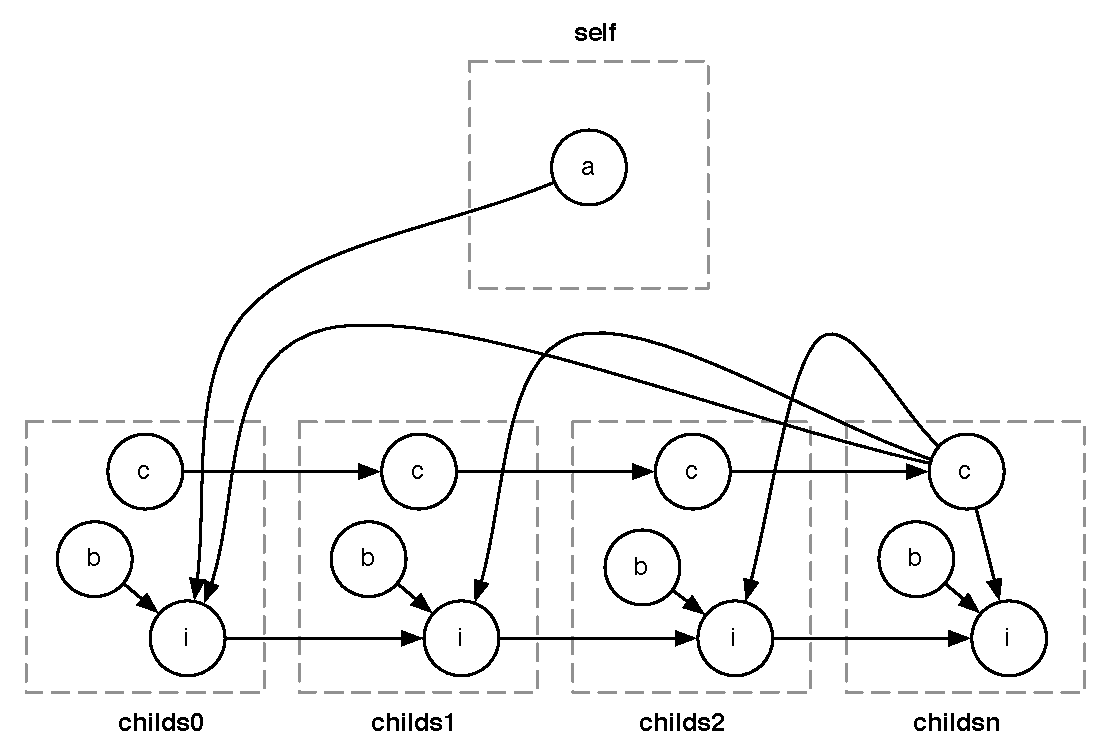
\includegraphics[trim=0 0 0 0,clip,width=0.7\columnwidth]{chapter3/unrolledloop}
\end{minipage}}\\
\subfloat[\textbf{Staging as Two Loops.}]{\label{fig:unrolling:stages}
\begin{minipage}{1\columnwidth}\centering
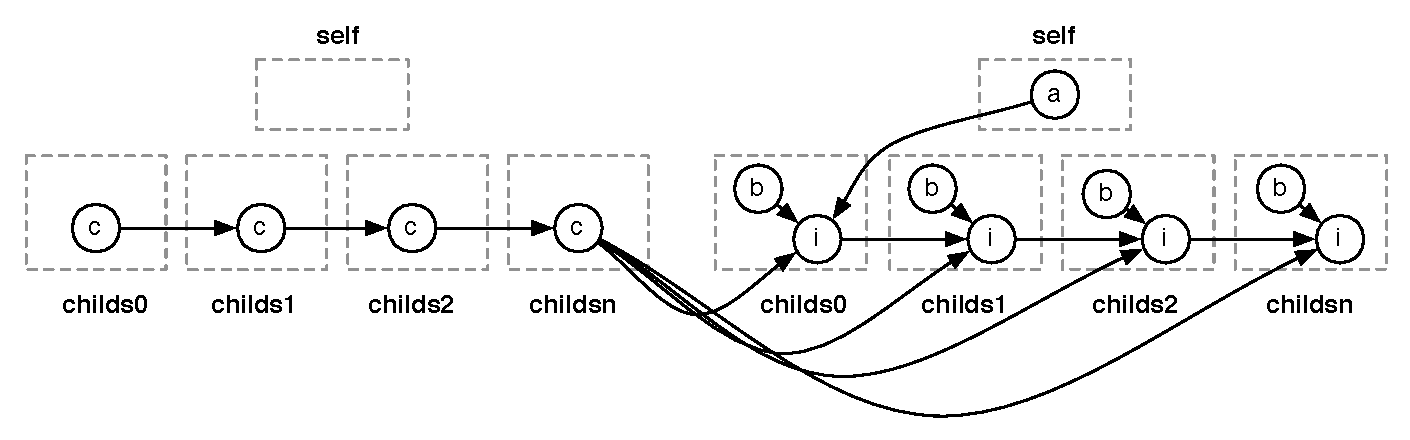
\includegraphics[trim=0 0 0 0,clip,width=1.0\columnwidth]{chapter3/stagedloop}
\end{minipage}}
\caption{\textbf{Loop scheduling}.The loop code can be scheduled as two loops that occur in the same traversal.}
\label{fig:unrolling}
\end{figure}



\subsection{Reduction to OAGs by Unrolling}
We show how to schedule the following loop:

\begin{lstlisting}[mathescape]
interface NodeI {
  var c : int;
  var i : int;
  input a : int;
  input b : int;
}
class NodeC : NodeI {
  children {  childs : [ NodeI ]; }
  actions {
    loop childs {
      childs.c := fold 0 .. childs$\$-$.c + 1;
      childs.i := 
        fold 
        a 
        ..         
        childs$\$-$.i  + childs$\$i$.b + childs$\$$.c;
    }
  }
}
\end{lstlisting}

Our reduction unrolls the loop into 4 steps ($0$, $1$, $2$, and $n$):

\begin{lstlisting}[mathescape]
interface NodeI {
  var c : int;
  var i : int;
  input a : int;
  input b : int;
}
class NodeC : NodeI {
  children {  
    childs0, childs1, childs2, childsn : NodeI;
  }
  actions {   
    childs0.c := 0 + 1;
    childs1.c := childs0.c + 1;
    childs2.c := childs1.c + 1;
    childsn.c := childs2.c + 1;

    childs0.i := a + childs0.b + childsn.c;
    childs1.i := childs0.i + childs1.b + childsn.c;
    childs2.i := childs1.i + childs2.b + childsn.c;
    childsn.i := childs2.i + childsn.b + childsn.c;
  }
}        
\end{lstlisting}



The reduction performs several rewrites that unroll loops and then substitute variable names in the unrolled statements:

\begin{figure}
\begin{align*}
\llbracket ~child : [ interface ] ~\rrbracket &\rightarrow child0, child1, child2, child \texttt{n} : interface 
\\
\llbracket child.fld := \texttt{fold} ~ e_{\texttt{init},fld} ~ .. ~ e_\texttt{step} \rrbracket &\rightarrow 
\\
& child0.fld = \llbracket~e_\texttt{step}[\forall ~f:  ~ e_{\texttt{init},f} ~/~ child\$\texttt{-}.f~]~\rrbracket_0; 
\\
& child1.fld = \llbracket~e_\texttt{step}~\rrbracket_1; 
\\
& child2.fld = \llbracket~e_\texttt{step}~\rrbracket_2; 
\\
& childn.fld = \llbracket~e_\texttt{step}~\rrbracket_\texttt{n} 
\\
\llbracket ~child\$\$.fld ~\rrbracket_\alpha &\rightarrow child \texttt{n}. fld
\\
\llbracket ~child\$i.fld \rrbracket_\alpha & \rightarrow child\alpha.fld
\\
\llbracket ~child\$\texttt{-}.fld \rrbracket_1 & \rightarrow child0.fld
\\
\llbracket ~child\$\texttt{-}.fld \rrbracket_2 & \rightarrow child1.fld
\\
\llbracket ~child\$\texttt{-}.fld \rrbracket_\texttt{n} & \rightarrow child2.fld
\end{align*}
\caption{\textbf{Rewrite Rules for Loop Reduction}. Cases of $\llbracket \cdot \rrbracket$ that simply recur are elided.}
\label{fig:loopreduction}
\end{figure}


\subsection{Recovery by Commuting Abstractions}





\section{Verification}

We automatically check an attribute grammar and its schedule for safety. This section focuses on two aspects of our approach: the properties to verify and the modular design of the verification procedure. The properties are significant in that they cover both functional and behavioral correctness, and are typically desired but not proven for layout languages and pattern programs. Furthermore, we check the properties through axiomatic reasoning parameterized by a local dependency analysis. This proof structure simplifies extending the language of statements and of schedules as most additions correspond to an isolated and com posable axiom. Later, in Chapter~\ref{chap:4}, we show a simple approach to changing the verifier into a synthesizer and thereby achieve fully automatic or computer-assisted parallelization.

Our approach automatically checks three properties. 
\begin{itemize}
\item \textbf{Totality} The specification defines one and only one solution for every well-formed input tree. 
\item \textbf{Determinism} The schedule evaluates the constraints of the attribute grammar without any data races.
\item \textbf{Linearity (Single Assignment)} Every attribute is assigned exactly once. Layout languages often perform \emph{reflow} to iteratively solve constraints or incremental computation, verifies that reflow is strictly an optimization.
\end{itemize}
In this chapter, we illustrate how to check race freedom. The check for linearity is similar , and totality is a consequence of the determinism and linearity properties.

We focus on a modular checking strategy for two reasons. First, we encountered implementation challenges without it. Our initial attempts to adapt the OAG~\cite{oag} algorithm, which is a search over a global dependency graph, suffered from many implementation bugs before we abandoned it. Our new approach instead decouples verification from synthesis and pattern checking from dependency analysis. Second, challenging our OAG implementation and the basic premise of our approach, we need to support adding new types of traversals. New schedule combinators, such as nested traversals, and individual patterns, such as recursive, should be simple to add as new types of parallel patterns are understood. Adding a parallel pattern should not require refactoring the entire verifier or synthesizer. Our new approach phrases each pattern as an independent axiom and automatically incorporates it into the checking procedure.



 \newcommand{\bigforall}[2]{{{\raisebox{-6pt}{\mbox{\Large$\forall$}$#1$}}\atop{\scriptstyle #2}}}

 


\begin{figure}[t]
\centering

$\begin{array}{c}
  $$\inference{ 
    \{ A \} ~p~ \{ B \} ~~~~~~~~ \{ B \} ~q~ \{ C \}
  }{ 
    \{ A \} ~p ~ ; ~ q~ \{ C \}
  }[  ]$$
\rrule{(seq)} \\ \vspace{1em} \\ 

$$\inference{ 
    \{ A \} ~p~ \{ B \} ~~~ \{ A \} ~q~ \{ C \}}{ 
    \{ A \} ~p ~ || ~ q~ \{ B \cup C \}
  }[ ]$$
\rrule{(par)} \\ \vspace{1em} \\

$$\inference{ 
Regions = \{\alpha \mapsto Visit*_\alpha\} ~ \cup ~ \displaystyle \bigcup_{i} \{\beta_i \mapsto Visit_i* \} \hfill \\
\forall~~ (\gamma \mapsto Visit*) \in Regions:  \hfill \\
~~~~ C_\gamma = \texttt{alwaysCommunicate}_\alpha(\gamma, B, Regions) \hfill \\
~~~~ \{ A, C_\gamma \} ~~ \gamma~Visit* ~~ \{ A \cup B_\gamma \} \hfill
}{ \{ A \} ~~ \alpha~  ~ Visit*_\alpha \{(\beta_i \mapsto Visit_i)* \}? ~~ \{ A \cup ~ \bigcup B_\gamma \} }[]$$
\rrule{(nest_\alpha)} \\ \vspace{1em} \\


$$\inference{
P = \cup Prod_i~~~~ Steps =  \cup Step_j \\
B = \displaystyle \bigcup_{i}\hfill\
\texttt{reachable}_\beta(Prod_i, P, A,Steps, C)}
{ \{ A , C \} ~~ \beta ~(Prod_i~\{~Step_j*~\})*  ~~ \{ A \cup B \}}[]$$
\rrule{(check_{\beta})} \\ \vspace{1em} %\\

%$$\inference{\{A\}~p~\{B\}~~~~ unify(sketch,p)}{\{ A \} ~ p \wedge sketch ~ \{ B \} }[]$$
%\rrule{(sketch)} 
\end{array}$  

%\begin{lstlisting}[mathescape]
%set unreachable($\beta$,$P$,$A$,$B$,$C$):
%  reachable := $\displaystyle \bigcup_{p \in P}$ reachable$_\beta$($p$, $A$, %$B$, $C$)
%  return B $-$ reachable
%\end{lstlisting}

\caption{Correctness axioms for checking a schedule}
\label{fig:deductions}
\end{figure}


\newsavebox{\parcheckers}
\begin{lrbox}{\parcheckers}% Store first listing
\begin{minipage}{1\columnwidth}
\centering
\begin{lstlisting}[mathescape,escapechar=\`,morekeywords={set,return}]
set reachable$_\texttt{parPre}$($W{\rightarrow}X$,$P$,$A$,$B$,$C$):  
  reach :=
    $~~~~ \{ a_{*,W{\rightarrow}X} ~ | ~ a_{*,W{\rightarrow}X}  \in A \} \cup~ (C \cap \{ a_{W,W{\rightarrow}X} ~ | \displaystyle \bigwedge _{V{\rightarrow}W \in P} W.a_{V{\rightarrow}W} \in B \}) \cup ~(C \cap \{ a_{X,W{\rightarrow}X}  ~ |  \neg \exists X{\rightarrow}Y \in P\})$
  while true:    
    progress := $\{ a_{*,W{\rightarrow}X} ~|~  a_{*,W{\rightarrow}X} = f(b_0, \ldots, b_n) \in \texttt{F}$ `\Suppressnumber` $\displaystyle \wedge ~ a_{*,W{\rightarrow}X} \in B ~ \wedge ~~ \bigwedge b_i \in ~$reach$\}$ `\Reactivatenumber`
    reach := reach $\cup$ progress
    if progress = $\emptyset$:
      break
  return reach  
\end{lstlisting}
\end{minipage}
\end{lrbox}

\newsavebox{\comcheckers}
\begin{lrbox}{\comcheckers}
\begin{minipage}{1\columnwidth}
\centering
\begin{lstlisting}[mathescape,escapechar=\`,morekeywords={set,return}]
$\texttt{alwaysCommunicate}_\texttt{parPre}(\beta, B, M) = \hfill$
  $\{ a_{W,W{\rightarrow}X} ~ | ~ (W{\rightarrow}X~B_\beta) \in M[\beta] ~~  \displaystyle \bigwedge _{(V{\rightarrow}W~B_\gamma) \in M[\gamma \neq \beta]}  a_{W,V{\rightarrow}W} \in B \cup A \} $
\end{lstlisting}

%\begin{lstlisting}[mathescape,escapechar=\`,morekeywords={set,return}]
%$\texttt{alwaysCommunicate}_\texttt{parPost}(\beta, B, M) = \hfill$
%  $\{ a_{X,W{\rightarrow}X} ~ | ~ (W{\rightarrow}X~B_\beta) \in M[\beta] $
%           $~ \wedge ~ \displaystyle \bigwedge _{(X{\rightarrow}Y~B_\gamma) \in M[\gamma %\neq \beta]}  a_{X,X{\rightarrow}Y} \in B \cup A \} $
%\end{lstlisting}


%\begin{lstlisting}[mathescape,escapechar=\`,morekeywords={set,return}]
%$\texttt{alwaysCommunicate}_\texttt{recursive} = %\texttt{alwaysCommunicate}_\texttt{parPre}$
%\end{lstlisting}

\end{minipage}
\end{lrbox}


\begin{figure}[t]
\subfloat[Communication check for region boundaries in a \sched{parPre} traversal]{
\label{fig:comm}
\usebox{\comcheckers}
} \\
\subfloat[ Unoptimized production visit check for \sched{parPre} traversal]{
\label{fig:parprecheck}
\usebox{\parcheckers}
}
\caption{Inter- and intra-region checkers for \sched{parPre}.}
\label{fig:checkers}
\end{figure}
 
 

\subsection{Axiomatic Correctness Checking}

%%%%%%

Correctness axioms for checking an entire schedule are in Figure~\ref{fig:deductions}. The judgements recursively check a composition of traversals until reaching the traversal-specific checks of Figure~\ref{fig:checkers}. Checking tames worst-case time linear in the number of attributes and the number of their local dependencies. As a reminder, Figure~\ref{fig:hboxparallel:decomplang} defines the language of schedules.

We use a small amount of notation. Variables $p$ and $q$ denote schedules (\lstinline{<Sched>}), $A$ and $B$ are sets of attributes, and $\alpha$ and $\beta$ are traversal types (\lstinline{<travAtomic>}). Attribute $a_{W, V{\rightarrow}W}$ is decorated with its production ($V{\rightarrow}W$) and the non-terminal within it ($W$). We write  $a_{*, V{\rightarrow}W}$ if $a$ can be associated with a non-terminal on either side of the production.

The rules to check composition and individual traversals are as follows:

\paragraph*{Sequential and parallel composition: ``\sched{;}'' and ``\sched{||}''}The simplest composition check is for sequencing: Hoare triple ``\sched{\{A\} p ; q \{C\}}'' (rule $\rrule{{seq}}$).  If attributes $A$ are solved before traversal ``\sched{p ; q}'', then attributes $C$ will be solved after. The conditions above the judgement bar state this is true if $p$ can always compute attributes $B$ given attributes $A$, and $q$ can always then compute $C$. The judgement is recursive. Analogous reasoning explains  ``\sched{||}'' (rule $\rrule{{par}}$).

%\paragraph*{}
%We split checking one traversal over the tree into two rules:

\paragraph*{Nested composition: $\mapsto$}
Rule $\rrule{{nest}_\alpha}$ checks outer traversal type $\alpha$ over regions where each one may have its own traversal type $\gamma$. Consider an outer traversal type of  \sched{parPre}: as it progresses top-down, every region might be guaranteed to have attributes of its root node solved before evaluation proceeds within it. For each region (the set of productions mapped to region traversal type $\gamma$), the rule calls $\texttt{alwaysCommunicate}_{\texttt{parPre}}$ to find the set $C_\gamma$ of  attributes that are externally set before the region is traversed. Rule $\rrule{{nest}_\alpha}$ calls checks for every region under the assumption that $C_\gamma$ is already solved.

The first line of rule $\rrule{{nest}_\alpha}$ means that, for any outer traversal $\alpha$, attributes scheduled for the outer region are  treated as if they were in their own region ($\gamma = \alpha$). Traversals that do not use nesting are degenerate:  all the productions belong to one region ($\gamma = \alpha$).

\paragraph*{Traversal over a region (e.g., parPre)}
The schedule for a traversal of type $\beta$ over a region is correct if every production visit schedule is correct (rule $\rrule{{check}_\beta}$). A production visit schedule $Prod_i~\{~Step_j*~\}$ is correct when there is an order for computing its scheduled attributes $Step_j*$ along which all of the data dependencies of the corresponding semantic functions are satisfied. %The order exists if the transitive closure of attributes with satisfiable dependencies covers $B$. 

Traversals that do not perform nesting, such as a single occurrence of \sched{parPre}, are handled as degenerate nested composition with one region: the entire tree.

\paragraph*{Production visit}

A fast and simple checking algorithm would be to mark each attribute  of a production as dirty or clean inside a structure that persists across checks of different visits to the same production. For each successive attribute in a visit's sequence, if all of its dependencies are met (dirty), mark the attribute, and otherwise fail the check. Non-local dependencies can be handled as below.


To optimize the synthesis algorithm of Chapter~\ref{chap:4}, we use a slightly indirect algorithm to check the correctness of visiting a production.  The intuition is that it relaxes the specification of visit's attributes by treating the ordered sequence as an unordered set and checks the reachability of the set's dependency graph. 

Figure~\frefb{fig:checkers}{fig:parprecheck} shows an unoptimized reachability computation for visiting a production inside a \sched{parPre} region. It is the standard transitive closure, except for two subtleties:

First, only attributes that are meant to be scheduled are considered reachable ($B$ membership check in line 7). Incorrectly including unscheduled attributes would erroneously allow attributes with unresolved dependencies to also be included.  

Second, attributes computed by visits to adjacent productions must be distinguished. Adjacent productions may be in the same region or in another. In a \sched{parPre} region, consider when $W$ is always an intermediate node of the region and attribute $a_{W,W{\rightarrow}X} \in B$ is always set by a parent production $V{\rightarrow}W$ in the same region. For this intra-region case, $a_{W,W{\rightarrow}X}$ is guaranteed to be reachable at the beginning of the visit to $W{\rightarrow}X$.  However, if $W$ can be the root node of the region, we must also check $a_{W,V{\rightarrow}W}$ is set by adjacent regions before the root is visited. %The checks for the intra-region case and the \texttt{alwaysCommunicate} inter-region case are in lines 4-5 of $\rrule{{nest}_\alpha}$.

%\paragraph*{Sketches}
%Rule $\rrule{{sketch}}$ separates checking the correctness of a schedule from whether a sketch matches it. First, a schedule must be correct irrespective of the accompanying sketch. Second, the schedule must syntactically match the schedule ($unify$). Later, we provide semantically constrained sketches that are checked by Prolog's more general unifier (Section~\ref{sec:prolog}). 

Checking an explicit sequence reduces to checking that the transitive closure can be performed in the specified order rather then the declarative definition in Figure~\ref{fig:checkers} . The synthesizer of Chapter~\ref{chap:4} does not need to check for ordering, so we omit this check.


%%%%%%
\subsection{Property Proofs}
The axioms check for determinism, which can be adapted to check the two other properties.

First, the axioms check determinism, which means that rerunning the schedule will yield the same result.  We can check determinism by ensuring that a schedule computes the attributes of an attribute grammar without races. More precisely, it tracks what attributes are guaranteed to have been computed by any particular point of the schedule, and uses that to check that every step of the computation only relies on what is guaranteed to have been computed.

Linearity requires that that every instance of an attribute is only assigned to once. We can check linearity by extending the axioms in two ways. First, they must check that for any given attribute $X_a$, it is either defined by all productions $X \rightarrow W$ or by all productions $W \rightarrow X$. Second, for every attribute assigned in production $X \rightarrow W$, it must only be scheduled for one visit. 

Totality guarantees that every well-formed input tree yields one and only one result. It is a property of the language because any schedule must reach the same result. In contrast, determinism is a property of a schedule because, for the same language, rerunning one schedule may always return the same result while the same might not be guaranteed for another schedule. The proof of totality lies in the proof of linearity. Given a linear schedule, the dynamic dependency graph of every input document is directed and acyclic. The DAG property guarantees that the value of each node is a pure function of the values of the dominating nodes, and therefore the language has a (total) functional interpretation. Checking totality adds an additional step beyond checking linearity: totality requires that every attribute in the grammar appears in the schedule.

\subsection{Verification is $O(|A|)$}
Verifying a schedule for race-freedom takes time linear in the number of attributes. Our  description of the checker in Figures~\ref{fig:deductions} and~\ref{fig:checkers} does not show the optimizations that lead to this bound so we highlight the key ideas here.

First, the number of axioms to check is linear in the number of attributes. Every traversal computes at least one attribute, which implies that the number of traversals is bounded by the number of attributes. Only non-empty visits must be checked, and their number is likewise bounded by the number of attributes.

Second, the time to check an axiom is linearly bounded by the number of attributes (and their dependencies) to be scheduled by that axiom. For example, checking the visit to a production is effectively a topological sort of the local dependency graph restricted to the attributes evaluated during the visit. Topologically sorting dependency graph $G = (E, V)$ is $O(|E| + |V|)$. An attribute can have at most $|A|$ local dependencies so verification takes time $O(|A|)$.  For simplicity, our implementation does not use the topological sort optimization, and we only encountered performance issues on one case study due to that.

Similar reasoning applies to quickly checking the two other properties. Linear checking of linearity follows the same proof structure. Each attribute is labeled based on the type of production that solves it and rule $\rrule{{check}_\beta}$ checks that the labels of attributes in $Step_j$ match production $Prod_i$. The time to check the axiom is therefore still bounded by the number of scheduled attributes. Finally, totality checks that the computed set of attributes matches the total set, and comparing two sets is also linear in the number of attributes.







\section{Evaluation: Layout as Structured Parallel Visits}
\subsection{Box model}
\subsection{Nested text}
\subsection{Grids}


\subsection{SIMD Rendering through Staged Memory Allocation}
We evaluate three dimensions of our staged memory allocation approach: flexibility, productivity, and performance. First, it needs to be able to express the rendering tasks that we encounter in GPU data visualization. Second, it should some form of productivity benefit for these tasks. Finally, the performance on those tasks must be fast  enough to support real-time animations and interactions of big data sets.



\subsubsection{Productivity}
Productivity is difficult to measure. Before using the automation extensions for rendering, we repeatedly encountered bugs in manipulating the allocation calls and memory buffers. The bugs related both to incorrect scheduling and to incorrect pointer arithmetic. Our new design eliminates the possibility of both bugs.

One suggestive productivity measure is of how many lines of code the macro abstraction eliminates from our visualizations. We measured the impact on using it for 3 of our visualizations. The first visualization is our HBox language extended with rendering calls, while the other two are interactive reimplementations of popular visualizations: a treemap~[[CITE]] and multiple 3D line graphs~[[CITE]].


\begin{table}[ht]
\caption{Lines of Code Before/After Invoking the '@' Macro}
\centering
\begin{tabular}{c r r r}
\hline\hline
 \textbf{Visualization} & \textbf{Before (loc)} & \textbf{After (loc)} & \textbf{Decrease} \\ [0.5ex] \hline
  HBox & 97 & 54 & 44\% \\
  Treemap & 296 & 241 & 19\% \\
  GE & 337 & 269 & 20\% \\ [1ex] 
\hline
\end{tabular}
\label{table:macroreduction}
\end{table}
Table~\ref{table:macroreduction} compares the lines of code in visualizations before and after we added the macros. Using the macros eliminated 19--44\% of the code. Note that we are \emph{not} measuring the macro-expanded code, but code that a human wrote.



As shown in Figure~\ref{fig:stagedallocClient}, the eliminated code is code that was introduced by staging the library calls. Porting unstaged functional graphics calls to the library, is in practice, an alpha renaming of function names.  Using the '@' macro eliminates 19--44\% of the code that would have otherwise been introduced and completely eliminates two classes of bugs (scheduling and pointer arithmetic), so the productivity benefit is non-trivial. 

\subsubsection{Performance}


\section{Related Work}
Lang of schedules
\begin{itemize}
\item background
\item stencils and skeletons: wavefront, ...
\item polyhedra
\end{itemize}
Schedule verification
\begin{itemize}
\item compare to OAG etc., looser dataflow/functional langs
\end{itemize}